

\tikzset{every picture/.style={line width=0.75pt}} %set default line width to 0.75pt

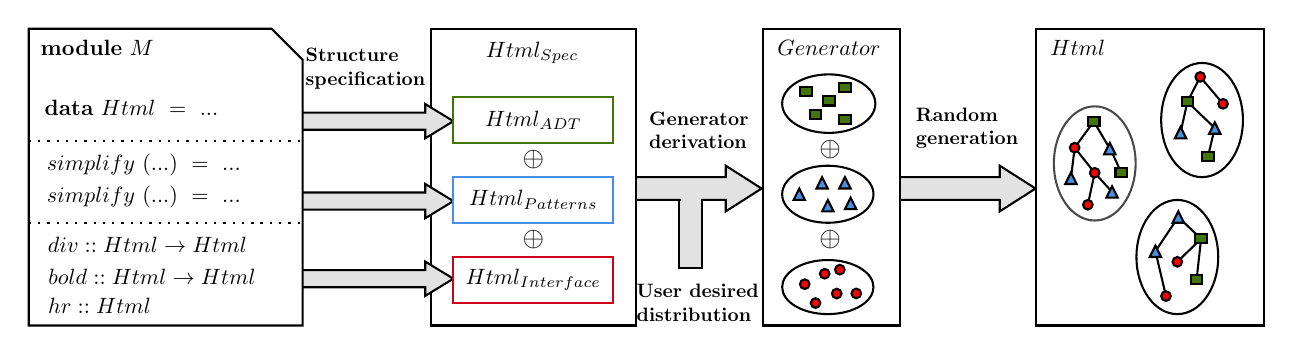
\begin{tikzpicture}[x=0.75pt,y=0.75pt,yscale=-1.1,xscale=1.1]
%uncomment if require: \path (0,439.4285583496094); %set diagram left start at 0, and has height of 439.4285583496094

%Right Arrow [id:dp7732858674364509]
\draw  [fill={rgb, 255:red, 226; green, 226; blue, 226 }  ,fill opacity=1 ] (340,230) -- (340,195) -- (335,195) -- (345,195) -- (355,195) -- (350,195) -- (350,230) -- cycle ;
%Right Arrow [id:dp2590973168233759]
\draw  [fill={rgb, 255:red, 226; green, 226; blue, 226 }  ,fill opacity=1 ] (311,190) -- (360.31,190) -- (360.31,185) -- (376,195) -- (360.31,205) -- (360.31,200) -- (311,200) -- cycle ;
%Shape: Rectangle [id:dp2141233912633571]
\draw  [fill={rgb, 255:red, 255; green, 255; blue, 255 }  ,fill opacity=1 ] (231,125) -- (321,125) -- (321,255) -- (231,255) -- cycle ;
%Right Arrow [id:dp06215174722463401]
\draw  [fill={rgb, 255:red, 226; green, 226; blue, 226 }  ,fill opacity=1 ] (171,161.75) -- (228.69,161.75) -- (228.69,158) -- (241,165.5) -- (228.69,173) -- (228.69,169.25) -- (171,169.25) -- cycle ;
%Right Arrow [id:dp6766910698477273]
\draw  [fill={rgb, 255:red, 226; green, 226; blue, 226 }  ,fill opacity=1 ] (171,196.75) -- (228.69,196.75) -- (228.69,193) -- (241,200.5) -- (228.69,208) -- (228.69,204.25) -- (171,204.25) -- cycle ;
%Right Arrow [id:dp3196923724356615]
\draw  [fill={rgb, 255:red, 226; green, 226; blue, 226 }  ,fill opacity=1 ] (171,230.75) -- (228.69,230.75) -- (228.69,227) -- (241,234.5) -- (228.69,242) -- (228.69,238.25) -- (171,238.25) -- cycle ;
%Right Arrow [id:dp0360549353694295]
\draw  [fill={rgb, 255:red, 226; green, 226; blue, 226 }  ,fill opacity=1 ] (431,190) -- (480.31,190) -- (480.31,185) -- (496,195) -- (480.31,205) -- (480.31,200) -- (431,200) -- cycle ;
%Shape: Rectangle [id:dp2934677500856828]
\draw  [fill={rgb, 255:red, 255; green, 255; blue, 255 }  ,fill opacity=1 ] (496,125) -- (596,125) -- (596,255) -- (496,255) -- cycle ;
%Straight Lines [id:da7152551743774183]
\draw    (558.5,207.5) -- (568.5,217) ;


%Straight Lines [id:da3837250992572381]
\draw    (558.5,207.5) -- (548.5,222.5) ;


%Straight Lines [id:da8680015881494354]
\draw    (568.5,217) -- (558.08,227.11) ;


%Straight Lines [id:da7327748351239962]
\draw    (548.5,222.5) -- (553.11,242.11) ;


%Straight Lines [id:da007641890318750955]
\draw    (568.5,217) -- (566.5,235) ;


%Straight Lines [id:da995333968066006]
\draw    (568.11,146.11) -- (578.11,157.89) ;


%Straight Lines [id:da015868138489393502]
\draw    (568.11,146.11) -- (562.5,157) ;


%Straight Lines [id:da7302160362706243]
\draw    (562.5,157) -- (574.5,168.5) ;


%Straight Lines [id:da46726020734917606]
\draw    (562.5,157) -- (559.5,170.5) ;


%Straight Lines [id:da4868124795808251]
\draw    (574.5,168.5) -- (571.5,181) ;


%Straight Lines [id:da6000768704792225]
\draw    (521.89,188.11) -- (529.5,196.5) ;


%Straight Lines [id:da9056461286434507]
\draw    (521.89,188.11) -- (518.89,202.11) ;


%Straight Lines [id:da5328270203547492]
\draw    (529,178.13) -- (533.5,188) ;


%Straight Lines [id:da38335809761139505]
\draw    (521.5,165.63) -- (528.5,177.5) ;


%Straight Lines [id:da39066239946769477]
\draw    (513.11,177.11) -- (521.89,188.11) ;


%Straight Lines [id:da6974822807110195]
\draw    (513.11,177.11) -- (511.5,190.5) ;


%Straight Lines [id:da06361852802164258]
\draw    (521.5,165.63) -- (513.11,177.11) ;


%Snip Single Corner Rect [id:dp4647891928859724]
\draw  [fill={rgb, 255:red, 255; green, 255; blue, 255 }  ,fill opacity=1 ] (55,125) -- (161.34,125) -- (175,138.66) -- (175,255) -- (55,255) -- cycle ;
%Shape: Rectangle [id:dp3811163355625795]
\draw  [fill={rgb, 255:red, 255; green, 255; blue, 255 }  ,fill opacity=1 ] (376.5,125) -- (436.5,125) -- (436.5,255) -- (376.5,255) -- cycle ;
%Shape: Ellipse [id:dp7838604577819246]
\draw   (385,238.16) .. controls (385,231.62) and (393.95,226.32) .. (405,226.32) .. controls (416.05,226.32) and (425,231.62) .. (425,238.16) .. controls (425,244.7) and (416.05,250) .. (405,250) .. controls (393.95,250) and (385,244.7) .. (385,238.16) -- cycle ;
%Shape: Circle [id:dp36073479073960346]
\draw  [color={rgb, 255:red, 0; green, 0; blue, 0 }  ,draw opacity=1 ][fill={rgb, 255:red, 255; green, 0; blue, 0 }  ,fill opacity=1 ] (408.16,230.53) .. controls (408.16,229.36) and (409.1,228.42) .. (410.26,228.42) .. controls (411.43,228.42) and (412.37,229.36) .. (412.37,230.53) .. controls (412.37,231.69) and (411.43,232.63) .. (410.26,232.63) .. controls (409.1,232.63) and (408.16,231.69) .. (408.16,230.53) -- cycle ;
%Shape: Circle [id:dp8080098028480491]
\draw  [color={rgb, 255:red, 0; green, 0; blue, 0 }  ,draw opacity=1 ][fill={rgb, 255:red, 255; green, 0; blue, 0 }  ,fill opacity=1 ] (397.53,245.16) .. controls (397.53,244) and (398.47,243.05) .. (399.63,243.05) .. controls (400.79,243.05) and (401.74,244) .. (401.74,245.16) .. controls (401.74,246.32) and (400.79,247.26) .. (399.63,247.26) .. controls (398.47,247.26) and (397.53,246.32) .. (397.53,245.16) -- cycle ;
%Shape: Circle [id:dp12076525384098513]
\draw  [color={rgb, 255:red, 0; green, 0; blue, 0 }  ,draw opacity=1 ][fill={rgb, 255:red, 255; green, 0; blue, 0 }  ,fill opacity=1 ] (415.37,240.95) .. controls (415.37,239.78) and (416.31,238.84) .. (417.47,238.84) .. controls (418.64,238.84) and (419.58,239.78) .. (419.58,240.95) .. controls (419.58,242.11) and (418.64,243.05) .. (417.47,243.05) .. controls (416.31,243.05) and (415.37,242.11) .. (415.37,240.95) -- cycle ;
%Shape: Ellipse [id:dp5212893057388461]
\draw  [color={rgb, 255:red, 0; green, 0; blue, 0 }  ,draw opacity=1 ][fill={rgb, 255:red, 255; green, 0; blue, 0 }  ,fill opacity=1 ] (401.53,232.32) .. controls (401.53,231.15) and (402.47,230.21) .. (403.63,230.21) .. controls (404.79,230.21) and (405.74,231.15) .. (405.74,232.32) .. controls (405.74,233.48) and (404.79,234.42) .. (403.63,234.42) .. controls (402.47,234.42) and (401.53,233.48) .. (401.53,232.32) -- cycle ;
%Shape: Circle [id:dp23843560123656338]
\draw  [color={rgb, 255:red, 0; green, 0; blue, 0 }  ,draw opacity=1 ][fill={rgb, 255:red, 255; green, 0; blue, 0 }  ,fill opacity=1 ] (406.79,241) .. controls (406.79,239.84) and (407.73,238.89) .. (408.89,238.89) .. controls (410.06,238.89) and (411,239.84) .. (411,241) .. controls (411,242.16) and (410.06,243.11) .. (408.89,243.11) .. controls (407.73,243.11) and (406.79,242.16) .. (406.79,241) -- cycle ;
%Shape: Ellipse [id:dp4809698571086918]
\draw   (385,197.5) .. controls (385,190.6) and (393.95,185) .. (405,185) .. controls (416.05,185) and (425,190.6) .. (425,197.5) .. controls (425,204.4) and (416.05,210) .. (405,210) .. controls (393.95,210) and (385,204.4) .. (385,197.5) -- cycle ;
%Shape: Triangle [id:dp24226788884090933]
\draw  [fill={rgb, 255:red, 74; green, 144; blue, 226 }  ,fill opacity=1 ] (392.5,195) -- (395,200) -- (390,200) -- cycle ;
%Shape: Triangle [id:dp5291497962409548]
\draw  [fill={rgb, 255:red, 74; green, 144; blue, 226 }  ,fill opacity=1 ] (402.5,190) -- (405,195) -- (400,195) -- cycle ;
%Shape: Triangle [id:dp5917974674439683]
\draw  [fill={rgb, 255:red, 74; green, 144; blue, 226 }  ,fill opacity=1 ] (412.5,190) -- (415,195) -- (410,195) -- cycle ;
%Shape: Triangle [id:dp29519879870465426]
\draw  [fill={rgb, 255:red, 74; green, 144; blue, 226 }  ,fill opacity=1 ] (405,200) -- (407.5,205) -- (402.5,205) -- cycle ;
%Shape: Triangle [id:dp6574937894365762]
\draw  [fill={rgb, 255:red, 74; green, 144; blue, 226 }  ,fill opacity=1 ] (415,199) -- (417.5,204) -- (412.5,204) -- cycle ;
%Shape: Ellipse [id:dp8770682879482239]
\draw   (385,157.81) .. controls (385,150.74) and (394.14,145) .. (405.42,145) .. controls (416.69,145) and (425.83,150.74) .. (425.83,157.81) .. controls (425.83,164.89) and (416.69,170.63) .. (405.42,170.63) .. controls (394.14,170.63) and (385,164.89) .. (385,157.81) -- cycle ;
%Shape: Circle [id:dp5633637507570923]
\draw  [color={rgb, 255:red, 0; green, 0; blue, 0 }  ,draw opacity=1 ][fill={rgb, 255:red, 255; green, 0; blue, 0 }  ,fill opacity=1 ] (392.79,236.89) .. controls (392.79,235.73) and (393.73,234.79) .. (394.89,234.79) .. controls (396.06,234.79) and (397,235.73) .. (397,236.89) .. controls (397,238.06) and (396.06,239) .. (394.89,239) .. controls (393.73,239) and (392.79,238.06) .. (392.79,236.89) -- cycle ;
%Shape: Rectangle [id:dp853277524439841]
\draw  [fill={rgb, 255:red, 65; green, 117; blue, 5 }  ,fill opacity=1 ] (397,160.63) -- (402,160.63) -- (402,164.63) -- (397,164.63) -- cycle ;
%Shape: Rectangle [id:dp26443574867732256]
\draw  [fill={rgb, 255:red, 65; green, 117; blue, 5 }  ,fill opacity=1 ] (393,150.63) -- (398,150.63) -- (398,154.63) -- (393,154.63) -- cycle ;
%Shape: Rectangle [id:dp3935753971313367]
\draw  [fill={rgb, 255:red, 65; green, 117; blue, 5 }  ,fill opacity=1 ] (410,148.63) -- (415,148.63) -- (415,152.63) -- (410,152.63) -- cycle ;
%Shape: Rectangle [id:dp5931653318550618]
\draw  [fill={rgb, 255:red, 65; green, 117; blue, 5 }  ,fill opacity=1 ] (410,162.63) -- (415,162.63) -- (415,166.63) -- (410,166.63) -- cycle ;
%Shape: Rectangle [id:dp7233342352369083]
\draw  [fill={rgb, 255:red, 65; green, 117; blue, 5 }  ,fill opacity=1 ] (403,154.63) -- (408,154.63) -- (408,158.63) -- (403,158.63) -- cycle ;
%Shape: Ellipse [id:dp9722655375449147]
\draw   (540.17,225) .. controls (540.17,211.19) and (548.19,200) .. (558.08,200) .. controls (567.98,200) and (576,211.19) .. (576,225) .. controls (576,238.81) and (567.98,250) .. (558.08,250) .. controls (548.19,250) and (540.17,238.81) .. (540.17,225) -- cycle ;
%Shape: Ellipse [id:dp9371514401907413]
\draw  [color={rgb, 255:red, 74; green, 74; blue, 74 }  ,draw opacity=1 ] (504,184) .. controls (504,170.19) and (512.02,159) .. (521.92,159) .. controls (531.81,159) and (539.83,170.19) .. (539.83,184) .. controls (539.83,197.81) and (531.81,209) .. (521.92,209) .. controls (512.02,209) and (504,197.81) .. (504,184) -- cycle ;
%Shape: Ellipse [id:dp26883422845191607]
\draw   (551,165) .. controls (551,151.19) and (559.02,140) .. (568.92,140) .. controls (578.81,140) and (586.83,151.19) .. (586.83,165) .. controls (586.83,178.81) and (578.81,190) .. (568.92,190) .. controls (559.02,190) and (551,178.81) .. (551,165) -- cycle ;
%Shape: Rectangle [id:dp5872203962807194]
\draw  [fill={rgb, 255:red, 65; green, 117; blue, 5 }  ,fill opacity=1 ] (519,163.63) -- (524,163.63) -- (524,167.63) -- (519,167.63) -- cycle ;
%Shape: Circle [id:dp7605266721377453]
\draw  [color={rgb, 255:red, 0; green, 0; blue, 0 }  ,draw opacity=1 ][fill={rgb, 255:red, 255; green, 0; blue, 0 }  ,fill opacity=1 ] (511,177.11) .. controls (511,175.94) and (511.94,175) .. (513.11,175) .. controls (514.27,175) and (515.21,175.94) .. (515.21,177.11) .. controls (515.21,178.27) and (514.27,179.21) .. (513.11,179.21) .. controls (511.94,179.21) and (511,178.27) .. (511,177.11) -- cycle ;
%Shape: Triangle [id:dp4125869850828281]
\draw  [fill={rgb, 255:red, 74; green, 144; blue, 226 }  ,fill opacity=1 ] (511.5,188) -- (514,193) -- (509,193) -- cycle ;
%Shape: Triangle [id:dp09394805352485558]
\draw  [fill={rgb, 255:red, 74; green, 144; blue, 226 }  ,fill opacity=1 ] (528.5,175) -- (531,180) -- (526,180) -- cycle ;
%Shape: Circle [id:dp7834832784546726]
\draw  [color={rgb, 255:red, 0; green, 0; blue, 0 }  ,draw opacity=1 ][fill={rgb, 255:red, 255; green, 0; blue, 0 }  ,fill opacity=1 ] (516.79,202.11) .. controls (516.79,200.94) and (517.73,200) .. (518.89,200) .. controls (520.06,200) and (521,200.94) .. (521,202.11) .. controls (521,203.27) and (520.06,204.21) .. (518.89,204.21) .. controls (517.73,204.21) and (516.79,203.27) .. (516.79,202.11) -- cycle ;
%Shape: Rectangle [id:dp18557164533567394]
\draw  [fill={rgb, 255:red, 65; green, 117; blue, 5 }  ,fill opacity=1 ] (531,186) -- (536,186) -- (536,190) -- (531,190) -- cycle ;
%Shape: Circle [id:dp8025931154410937]
\draw  [color={rgb, 255:red, 0; green, 0; blue, 0 }  ,draw opacity=1 ][fill={rgb, 255:red, 255; green, 0; blue, 0 }  ,fill opacity=1 ] (519.79,188.11) .. controls (519.79,186.94) and (520.73,186) .. (521.89,186) .. controls (523.06,186) and (524,186.94) .. (524,188.11) .. controls (524,189.27) and (523.06,190.21) .. (521.89,190.21) .. controls (520.73,190.21) and (519.79,189.27) .. (519.79,188.11) -- cycle ;
%Shape: Triangle [id:dp1239939418024707]
\draw  [fill={rgb, 255:red, 74; green, 144; blue, 226 }  ,fill opacity=1 ] (529.5,194) -- (532,199) -- (527,199) -- cycle ;
%Shape: Circle [id:dp8812473863475445]
\draw  [color={rgb, 255:red, 0; green, 0; blue, 0 }  ,draw opacity=1 ][fill={rgb, 255:red, 255; green, 0; blue, 0 }  ,fill opacity=1 ] (566,146.11) .. controls (566,144.94) and (566.94,144) .. (568.11,144) .. controls (569.27,144) and (570.21,144.94) .. (570.21,146.11) .. controls (570.21,147.27) and (569.27,148.21) .. (568.11,148.21) .. controls (566.94,148.21) and (566,147.27) .. (566,146.11) -- cycle ;
%Shape: Circle [id:dp7598993443376705]
\draw  [color={rgb, 255:red, 0; green, 0; blue, 0 }  ,draw opacity=1 ][fill={rgb, 255:red, 255; green, 0; blue, 0 }  ,fill opacity=1 ] (576,157.89) .. controls (576,156.73) and (576.94,155.79) .. (578.11,155.79) .. controls (579.27,155.79) and (580.21,156.73) .. (580.21,157.89) .. controls (580.21,159.06) and (579.27,160) .. (578.11,160) .. controls (576.94,160) and (576,159.06) .. (576,157.89) -- cycle ;
%Shape: Rectangle [id:dp3435681036136593]
\draw  [fill={rgb, 255:red, 65; green, 117; blue, 5 }  ,fill opacity=1 ] (560,155) -- (565,155) -- (565,159) -- (560,159) -- cycle ;
%Shape: Triangle [id:dp4971718332882904]
\draw  [fill={rgb, 255:red, 74; green, 144; blue, 226 }  ,fill opacity=1 ] (559.5,168) -- (562,173) -- (557,173) -- cycle ;
%Shape: Triangle [id:dp8772068767151546]
\draw  [fill={rgb, 255:red, 74; green, 144; blue, 226 }  ,fill opacity=1 ] (574.5,166) -- (577,171) -- (572,171) -- cycle ;
%Shape: Rectangle [id:dp5389313915531764]
\draw  [fill={rgb, 255:red, 65; green, 117; blue, 5 }  ,fill opacity=1 ] (569,179) -- (574,179) -- (574,183) -- (569,183) -- cycle ;
%Shape: Triangle [id:dp9780900800848462]
\draw  [fill={rgb, 255:red, 74; green, 144; blue, 226 }  ,fill opacity=1 ] (558.5,205) -- (561,210) -- (556,210) -- cycle ;
%Shape: Triangle [id:dp6412646282331236]
\draw  [fill={rgb, 255:red, 74; green, 144; blue, 226 }  ,fill opacity=1 ] (548.5,220) -- (551,225) -- (546,225) -- cycle ;
%Shape: Rectangle [id:dp6641116065775097]
\draw  [fill={rgb, 255:red, 65; green, 117; blue, 5 }  ,fill opacity=1 ] (566,215) -- (571,215) -- (571,219) -- (566,219) -- cycle ;
%Shape: Circle [id:dp09340888622817034]
\draw  [color={rgb, 255:red, 0; green, 0; blue, 0 }  ,draw opacity=1 ][fill={rgb, 255:red, 255; green, 0; blue, 0 }  ,fill opacity=1 ] (555.98,227.11) .. controls (555.98,225.94) and (556.92,225) .. (558.08,225) .. controls (559.25,225) and (560.19,225.94) .. (560.19,227.11) .. controls (560.19,228.27) and (559.25,229.21) .. (558.08,229.21) .. controls (556.92,229.21) and (555.98,228.27) .. (555.98,227.11) -- cycle ;
%Shape: Circle [id:dp14489754689178413]
\draw  [color={rgb, 255:red, 0; green, 0; blue, 0 }  ,draw opacity=1 ][fill={rgb, 255:red, 255; green, 0; blue, 0 }  ,fill opacity=1 ] (551,242.11) .. controls (551,240.94) and (551.94,240) .. (553.11,240) .. controls (554.27,240) and (555.21,240.94) .. (555.21,242.11) .. controls (555.21,243.27) and (554.27,244.21) .. (553.11,244.21) .. controls (551.94,244.21) and (551,243.27) .. (551,242.11) -- cycle ;
%Shape: Rectangle [id:dp1568842876109131]
\draw  [fill={rgb, 255:red, 65; green, 117; blue, 5 }  ,fill opacity=1 ] (564,233) -- (569,233) -- (569,237) -- (564,237) -- cycle ;
%Straight Lines [id:da9505573863907721]
\draw  [dash pattern={on 0.84pt off 2.51pt}]  (55,210) -- (175,210) ;


%Straight Lines [id:da9881747537161369]
\draw  [dash pattern={on 0.84pt off 2.51pt}]  (55,174) -- (175,174) ;


%Shape: Rectangle [id:dp7912203503474478]
\draw  [color={rgb, 255:red, 65; green, 117; blue, 5 }  ,draw opacity=1 ][fill={rgb, 255:red, 255; green, 255; blue, 255 }  ,fill opacity=1 ] (241,155) -- (311,155) -- (311,175) -- (241,175) -- cycle ;
%Shape: Rectangle [id:dp4628817838994279]
\draw  [color={rgb, 255:red, 208; green, 2; blue, 27 }  ,draw opacity=1 ][fill={rgb, 255:red, 255; green, 255; blue, 255 }  ,fill opacity=1 ] (241,225) -- (311,225) -- (311,245) -- (241,245) -- cycle ;

%Shape: Rectangle [id:dp14183247266409804]
\draw  [color={rgb, 255:red, 74; green, 144; blue, 226 }  ,draw opacity=1 ][fill={rgb, 255:red, 255; green, 255; blue, 255 }  ,fill opacity=1 ] (241,190) -- (311,190) -- (311,210) -- (241,210) -- cycle ;

%Straight Lines [id:da20016875561182368]
\draw [color={rgb, 255:red, 226; green, 226; blue, 226 }  ,draw opacity=1 ][line width=1.5]    (340.5,200) -- (349.5,200) ;



% Text Node
\draw (85,133.5) node [scale=0.8]  {$\text{\textbf{module}}\ M$};
% Text Node
\draw (100,159.5) node [scale=0.8]  {$\text{\textbf{data}}\ Html\ =\ ... $};
% Text Node
\draw (107,219.5) node [scale=0.8]  {$div::Html\rightarrow Html$};
% Text Node
\draw (109,233.5) node [scale=0.8]  {$bold::Html\rightarrow Html$};
% Text Node
\draw (86,246.5) node [scale=0.8]  {$hr::Html$};
% Text Node
\draw (275.5,135.5) node [scale=0.8]  {$Html_{Spec}$};
% Text Node
\draw (276,165) node [scale=0.8]  {$Html_{ADT}$};
% Text Node
\draw (276,200) node [scale=0.8]  {$Html_{Patterns}$};
% Text Node
\draw (276,235) node [scale=0.8]  {$Html_{Interface}$};
% Text Node
\draw (276,182.5) node   {$\boldsymbol{\oplus}$};
% Text Node
\draw (276,217.5) node   {$\boldsymbol{\oplus}$};
% Text Node
\draw (405.5,133.5) node [scale=0.8]  {$Generator$};
% Text Node
\draw (406,178) node   {$\boldsymbol{\oplus}$};
% Text Node
\draw (406,217.5) node   {$\boldsymbol{\oplus}$};
% Text Node
\draw (514.5,133.5) node [scale=0.8]  {$Html$};
% Text Node
\draw (107,184.5) node [scale=0.8]  {$simplify\ ( ...) \ =\ ... \ $};
% Text Node
\draw (107,198.5) node [scale=0.8]  {$simplify\ ( ...) \ =\ ... \ $};
% Text Node
\draw (202.5,142.5) node [scale=0.7] [align=left] {\textbf{Structure}\\ \textbf{specification}};
% Text Node
\draw (348.5,169.5) node [scale=0.7] [align=left] {\textbf{Generator}\\ \textbf{derivation}};
% Text Node
\draw (466,168.5) node [scale=0.7] [align=left] {\textbf{Random} \\ \textbf{generation}};
% Text Node
\draw (348,245) node [scale=0.7] [align=left] {\textbf{User desired} \\ \textbf{distribution}};


\end{tikzpicture}
